\begin{frame}
\frametitle{Measurement of  EDM in storage ring}
\framesubtitle{\textbf{\textbf{Protons at magic momentum in pure electric ring}}}


\vspace{-0.2cm}
\begin{block}{How to measure EDM of proton:}
	\begin{enumerate}
		\item Place polarized particles in a storage ring.
		\item Align spin along direction of flight at magic momentum. 
		\begin{itemize}
			\item[$\Rightarrow$] \textit{freeze} horizontal spin precession.
		\end{itemize}
		\item Search for time development of vertical polarization. 
	\end{enumerate}
\end{block}

\begin{columns}
	\column{0.35\textwidth}
	\hspace{0.3cm}
	\begin{tikzpicture}
	\node[anchor=south west,inner sep=0] (image) at (0,0) {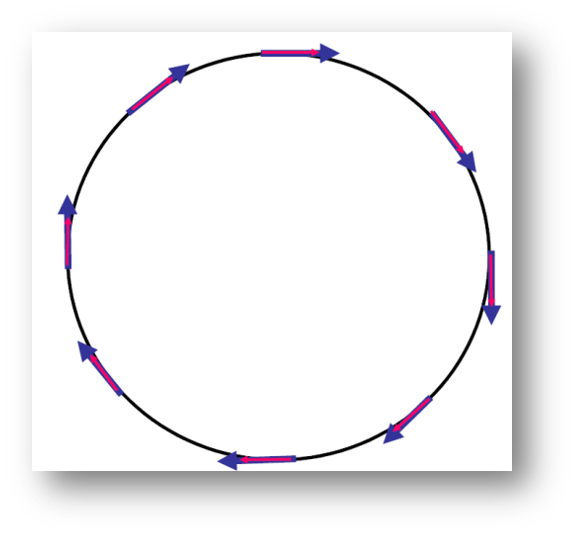
\includegraphics[width=0.8\textwidth]{frozen-spin.png}};
	\begin{scope}[x={(image.south east)},y={(image.north west)}]
	\draw (0.5,0.7)  node[font=\large] {$\vec \Omega = 0$};
	\draw (0.5,0.45)  node[font=\large] {$\displaystyle\frac{\dd \vec S}{\dd t} = \vec d \times \vec E$};
	\end{scope}
	\end{tikzpicture}
	\column{0.6\textwidth}
	\vspace{-0.3cm}
	\begin{figure}
		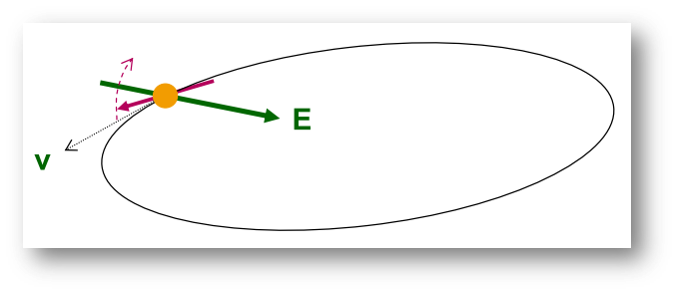
\includegraphics[width=1\textwidth]{polarization-buildup.png}
	\end{figure}
\end{columns}

\vspace{-0.3cm}
\begin{alertblock}{Storage ring method to measure EDMs of charged particles:}
	\begin{itemize}
		\item \textbf{Magic rings with spin frozen} along  momentum of particle.
		\item Polarization buildup $p_y(t)\propto d$.
	\end{itemize}
\end{alertblock}

\end{frame}
